This example was designed to introduce \bioptim's ability to reduce the number of degrees-of-freedom (DoF) of a model via the \texttt{BiMapping} feature, to account for nonlinear boundaries on the controls, and to solve complex multiphase programs.
A total of five phases were used to describe the various dynamics of the jump, namely the push-off phase (i.e., flat foot (two floor contacts\footnote{A contact is defined as a point where forces are applied to cancel its acceleration.}) and then toe only (one contact)), flight (free fall, i.e., no contact) and landing (toe (one contact) and then flat foot (two contacts)).
The transitions between phases where contacts are added are approximated with the build-in inelastic impact \texttt{PhaseTransition.IMPACT}, which computes the velocity of the kinematic chain after an impact.
A pseudo-2D full-body symmetrized model consisting of 3~DoFs at the pelvis (forward and upward translations, tranverse rotation), 1~DoF at the upper limb (shoulder flexion), and 3~DoFs at the lower limb (hip, knee and ankle flexion) was used.
Since this is a full-body model, the root segment (i.e., the pelvis) was left uncontrolled, reducing the number of control variables to 4, namely the shoulder, hip, knee and ankle flexions. 
The objective function with the most important weight was a Mayer objective computed at the end of the push-off phase consisting in maximizing the jump height ($h$) from the free fall equations applied to the center of mass.
The remaining objective functions were regularization terms and terms that favoured a human-like solution. 
\[ 
  \resizebox{0.90\columnwidth}{!}{$ 
  \begin{aligned}
  \mathcal{J} = &~\underbrace{\omega_h~h}_{\mathtt{MIN\_PREDICTED\_COM\_HEIGHT}}~+~\underbrace{\omega_{x} \| \mathbf{\tilde{x}}(T_5) - \mathbf{\tilde{x}}^*\|^2}_{\mathtt{TRACK\_STATE}}\\
  +~&\sum^5_{i=1}~\underbrace{\omega_{t}(T_i - T_{i-1})}_{\mathtt{MIN\_TIME}}~
    +~\sum_{i=2}^4\int_{t=T_i}^{T_{i+1}}\underbrace{\omega_{sd}\left|\left|\frac{d\mathbf{\dot{q}}}{dt}\right|\right|^2}_{\mathtt{MIN\_STATE\_DERIVATIVE}}~dt
  \end{aligned}  
  $} 
  \addtag  
  \label{eq:cost_jumper}
\]
where $T_i$ with $i \in [1, 2, 3, 4, 5]$ are the final times of the i$^{th}$ phase respectively, and $T_0=0$; 
$\omega_h=-100$ is the weight of the jump height term defined negative to maximize it; 
$\omega_t=0.1$, $\omega_{sd}=0.1$ and $\omega_x=1.0$ are the weights of their respective objective functions; 
$\mathbf{\dot{q}}$ is the generalized velocities part of the state vector $\mathbf{x}$; 
and $\mathbf{\tilde{x}}$ is the state vector excluding the translations of the root segment. 
The $\mathbf{\tilde{x}}^*$ corresponds to a reference static position of the avatar with its knee slightly flexed and its arms horizontal.

Joint angles were bounded to human-like limits.
The first node of the first phase was enforced to be equal to $\mathbf{x^*}$ (i.e., including the translations of the root segment to be at the origin). 
Joint velocities were arbitrarily bounded to human-like limits.
Joint torques were bounded with nonlinear torque/angle/velocity relashionships measured on a high-level athlete using an isokinetic dynamometer. 
Non slipping (\texttt{NON\_SLIPPING}) and unilateral (\texttt{CONTACT\_FORCE}) contact force constraints were added to prevent the contact points from slipping and pulling on the ground.
During the ground phases, the heels had to remain over the floor.
To speed-up the solving with \emph{ipopt}, the problem was first solved using a BFGS Hessian approximation for 200 iterations.
Then, starting from this first solution, the problem was re-optimized, with the exact-Hessian computations.

\begin{figure}[t!]
  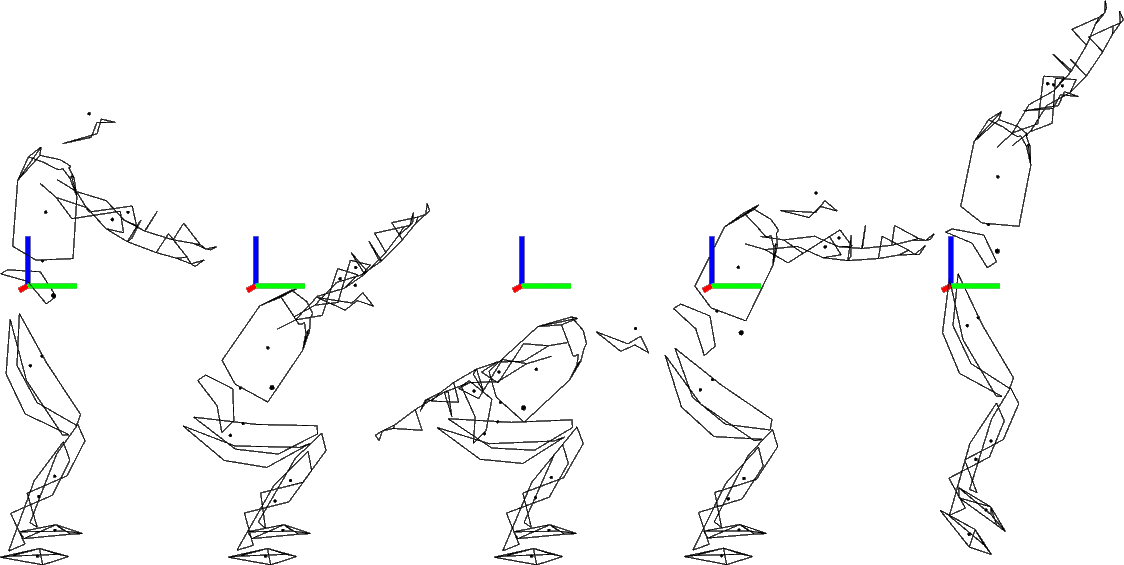
\includegraphics[width=\columnwidth]{figures/kinogramme_jump}
  \caption{Snapshots of the push-off phase of a vertical jump (Ex.~\ref{ex:jump}) where the avatar reproduces a human-like jump movement.} 
  \label{fig:jump}
\end{figure}

The optimized solution was obtained in 148 iterations of the exact-Hessian optimization \comment{for a total optimization time of $\SI{1780}{\second}$ ($\approx\SI{30}{\minute}$)}{A déplacer dans le tableau}, resulting in a \SI{1.28}{\meter} jump height.
The optimized time for the phases $1$ to $5$ were $0.70, 0.05, 0.99, 0.36, 0.21$ seconds, respectively.
The solution reproduced a human proximo-distal strategy (Fig~\ref{fig:jump}), i.e., activating large segments first (for instance the torso) and sequentially adding more distal segments, consequently ending up with the feet.
